\chapter{Implementation}

Implementations in the C programming language for the presented strategies can
be found in Appendix \ref{app:cimpl}. Although directly writing Assembler code
could result in a small performance benefit, this generally increases the work
necessary by an order of magnitude for only limited results. Instruction-level
optimization and in particular register allocation is left to the compiler.
Relying on the compiler mandates a closer study of the generated, optimized
assembler. All source files were compiled using clang version 15.0.7 and
optimization level O3.

\section{Pipelining}

Understanding certain choices requires an understanding of the Cortex-A73
instruction pipeline\cite{a72opt:2015}. Being a superscalar processor, it is
able to execute more than one instruction per clock cycle by dispatching
instructions to different execution units working in parallel.

\begin{figure}{h!}
    \centering
    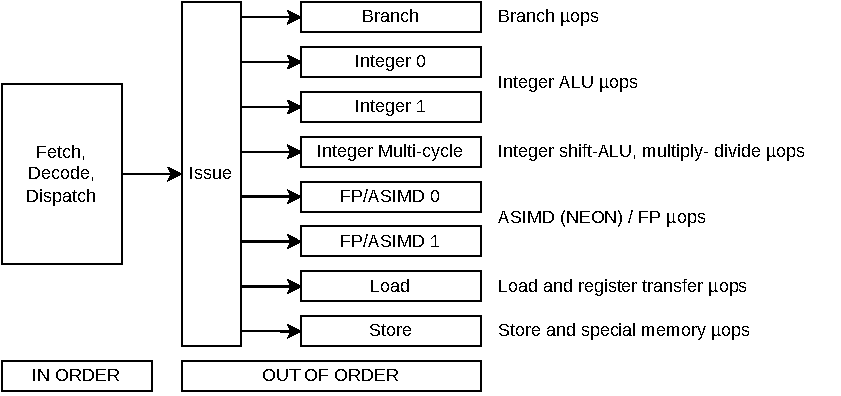
\includegraphics[width=0.7\textwidth]{Figures/a72pipeline.pdf}
    \caption{High-level overview of the Cortex-A72 instruction pipeline}
\end{figure}

The processor might for example store a calculation result, load a necessary
value from memory and execute two SIMD operations at once, all in the same
clock cycle. Modern compilers take advantage of this fact by reordering
instructions such that all pipeline execution units stay as busy as possible
and do not stall while having to wait for new instructions to be dispatched. A
more thorough analysis will be presented for the bitsliced strategy of
\texttt{GIFT}, but all implementations are heavily reliant on function
inlining, instruction reordering and loop unrolling.

\section{GIFT}
\subsection{Table-based}

This is the simplest strategy to implement. Indeed, its biggest advantage lies
in its portability to other platforms without relying on specific features or
extensions. The cipher state is stored as a 64-bit word and one round consists
in extracting the 4-bit S-boxes, looking up table values, collecting these in
an accumulator and finally adding the round key.

% TODO add bitfield extract explanation here

\lstinputlisting[language=c, firstline=77, lastline=87]{../impl/table/gift_table.c}
\lstinputlisting[language=c, firstline=89, lastline=101]{../impl/table/gift_table.c}

\subsection{Using \texttt{vperm}}

Implementation of the substitution layer requires the use of a single vector
intrinsic. This mandates the packing of data into a vector register which in
turn is disadvantageous to the permutation layer as we need to extract single
bits. Packing and unpacking is nothing more than filling 8-bit vector lanes
with 4-bit S-boxes and vice versa.

\lstinputlisting[language=c, firstline=92, lastline=95]{../impl/vector/gift_vec_sbox.c}
\lstinputlisting[language=c, firstline=102, lastline=117]{../impl/vector/gift_vec_sbox.c}
\lstinputlisting[language=c, firstline=197, lastline=212]{../impl/vector/gift_vec_sbox.c}

\subsection{Bitslicing}

We will examine the round function in closer detail and compare the source code
with the generated assembly.
\pagebreak

\begin{lstlisting}[language=c, caption={Round function src}]
for (int round = 0; round < ROUNDS_GIFT_64; round++) {
    gift_64_vec_sliced_subcells(s);
    gift_64_vec_sliced_permute(s);

    // round key addition
    s[0].val[0] = veorq_u8(s[0].val[0], rks[round][0].val[0]);
    s[0].val[1] = veorq_u8(s[0].val[1], rks[round][0].val[1]);
    s[0].val[2] = veorq_u8(s[0].val[2], rks[round][0].val[2]);
    s[0].val[3] = veorq_u8(s[0].val[3], rks[round][0].val[3]);
    s[1].val[0] = veorq_u8(s[1].val[0], rks[round][1].val[0]);
    s[1].val[1] = veorq_u8(s[1].val[1], rks[round][1].val[1]);
    s[1].val[2] = veorq_u8(s[1].val[2], rks[round][1].val[2]);
    s[1].val[3] = veorq_u8(s[1].val[3], rks[round][1].val[3]);
}
\end{lstlisting}

\begin{minipage}{.45\textwidth}
    \begin{lstlisting}[language={[ARM]Assembler}, caption={Round function asm}, escapechar=|]
and     v20.16b, v17.16b, v6.16b
add     x9, x20, x8
eor     v20.16b, v20.16b, v16.16b
add     x8, x8, #0x80|\label{lst:cntrincr}|
and     v21.16b, v20.16b, v19.16b
cmp     x8, #0xe70|\label{lst:cntrchk}|
eor     v21.16b, v21.16b, v6.16b
orr     v6.16b, v6.16b, v16.16b
eor     v6.16b, v6.16b, v17.16b
eor     v16.16b, v19.16b, v6.16b
eor     v17.16b, v16.16b, v20.16b
and     v19.16b, v21.16b, v17.16b
eor     v6.16b, v19.16b, v6.16b
and     v19.16b, v7.16b, v4.16b
eor     v19.16b, v19.16b, v5.16b
and     v20.16b, v19.16b, v18.16b
eor     v20.16b, v20.16b, v4.16b
orr     v4.16b, v4.16b, v5.16b
eor     v4.16b, v4.16b, v7.16b
eor     v5.16b, v18.16b, v4.16b
eor     v7.16b, v5.16b, v19.16b
and     v18.16b, v20.16b, v7.16b
eor     v4.16b, v18.16b, v4.16b
    \end{lstlisting}
\end{minipage}\hfill
\begin{minipage}{.45\textwidth}
    \vspace*{7mm}
    \begin{lstlisting}[language={[ARM]Assembler}, firstnumber=24, escapechar=|]
tbl     v18.16b, {v6.16b}, v2.16b
tbl     v19.16b, {v21.16b}, v3.16b
tbl     v21.16b, {v4.16b}, v2.16b
ldp     q6, q4, [x9, #-112]|\label{lst:floatload}|
mvn     v16.16b, v16.16b
tbl     v16.16b, {v16.16b}, v0.16b
tbl     v17.16b, {v17.16b}, v1.16b
mvn     v5.16b, v5.16b
tbl     v5.16b, {v5.16b}, v0.16b
ldp     q22, q23, [x9, #-80]
eor     v6.16b, v6.16b, v16.16b
eor     v16.16b, v4.16b, v17.16b
tbl     v7.16b, {v7.16b}, v1.16b
eor     v17.16b, v22.16b, v18.16b
tbl     v20.16b, {v20.16b}, v3.16b
ldp     q4, q18, [x9, #-48]
eor     v19.16b, v23.16b, v19.16b
eor     v4.16b, v4.16b, v5.16b
ldp     q22, q23, [x9, #-16]
eor     v5.16b, v18.16b, v7.16b
eor     v7.16b, v22.16b, v21.16b
eor     v18.16b, v23.16b, v20.16b
b.ne    197e0
    \end{lstlisting}
\end{minipage}

Without needing to dive too deep into details, it is obvious to see the
compiler has inlined the two function calls to \texttt{subcells} and
\texttt{permute} with lines 1 to 23 originating from the \texttt{subcells} and
lines 24-46 from the \texttt{permute} and round key addition functions. It has
chosen not to unroll the loop, but has moved the loop counter increment as well
as the condition check in between the \texttt{subcells} instructions to line
\ref{lst:cntrincr} and \ref{lst:cntrchk}. In addition, the loop counter serves
a second purpose as an offset register and is therefore incremented by 0x80=128
instead of just 1.

Permutation (\texttt{tbl}) and round key addition (\texttt{eor}) instructions
are interleaved. The compiler recognizes data dependencies and can therefore
proceed with round key addition immediately after a slice has been permuted
without needing to wait for all permutations to finish. This is only logical
considering the inner workings of the instruction pipeline: by interleaving
NEON with regular logic and load instructions, the execution units are filled
more evenly and pipeline stalls are prevented which speeds up computation.

Round keys are loaded from memory a few instructions before they are needed;
assuming all round keys are stored in the L1 cache, loading a
floating-point/vector register takes 5 cycles. After the load has been
dispatched to the load execution unit in line \ref{lst:floatload}, the
processor happily continues chugging away at the instruction stream by issuing
\texttt{tbl} and \texttt{mvn} $\mu$ops to other execution units.

These kinds of optimizations are pervasive when programming using higher level
languages like C and modern-day compilers more often than not outperform
handcrafted assembly.
